% This example is meant to be compiled with lualatex or xelatex

% The theme itself also supports pdflatex
\PassOptionsToPackage{unicode}{hyperref}
\documentclass[aspectratio=1610, 10pt]{beamer}

% Load packages you need here
\usepackage{polyglossia}
\setmainlanguage{english}
\usepackage[font=small,labelfont=bf]{caption}
\usepackage{csquotes}
\usepackage{siunitx}
\usepackage{subfigure}

\usepackage{amsmath}
\usepackage{amssymb}
\usepackage{mathtools}

\usepackage{hyperref}
\usepackage{bookmark}
\usepackage[absolute,overlay]{textpos}

%\usepackage[texcoord,
%grid,gridcolor=red!10,subgridcolor=green!10,gridunit=pt]
%{eso-pic}
% load the theme after all packages

\usetheme[
  showtotalframes, % show total number of frames in the footline
]{tudo}

% Put settings here, like
\unimathsetup{
  math-style=ISO,
  bold-style=ISO,
  nabla=upright,
  partial=upright,
  mathrm=sym,
}

\title{\Large{Cherenkov Detectors}}
\author[C.~Krause]{\normalsize{Christopher Krause \\
Key experiments in particle physics}}
%\institute[E4]{\normalsize{Experimentelle Physik IV} \\ \normalsize{Fakultät Physik}}
\titlegraphic{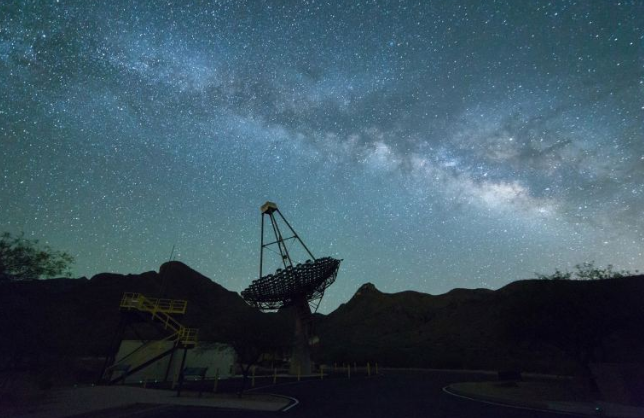
\includegraphics[width=0.53\textwidth]{images/title_picture.png}}


\begin{document}

\maketitle


\begin{frame}{Cherenkov radiation}
  \begin{itemize}
    \item Discovered by Pavel Cherenkov in 1934 around a radioactive preparation in water (1958 Nobel Prize)
    \item Theory was developed in 1937 by Igor Tamm and Ilya Frank (1958 Nobel Prize)
    \item Electromagnetic radiation of a dielectric medium, when a charged particle moves
    faster than the phase speed of light in that medium
  \end{itemize}
  \begin{figure}
      \subfigure[]{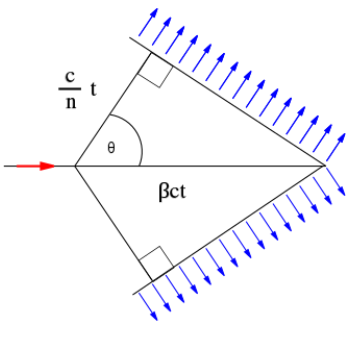
\includegraphics[width=0.25\textwidth]{images/cherenkov.PNG}}
      \hspace{1cm}
      \subfigure[]{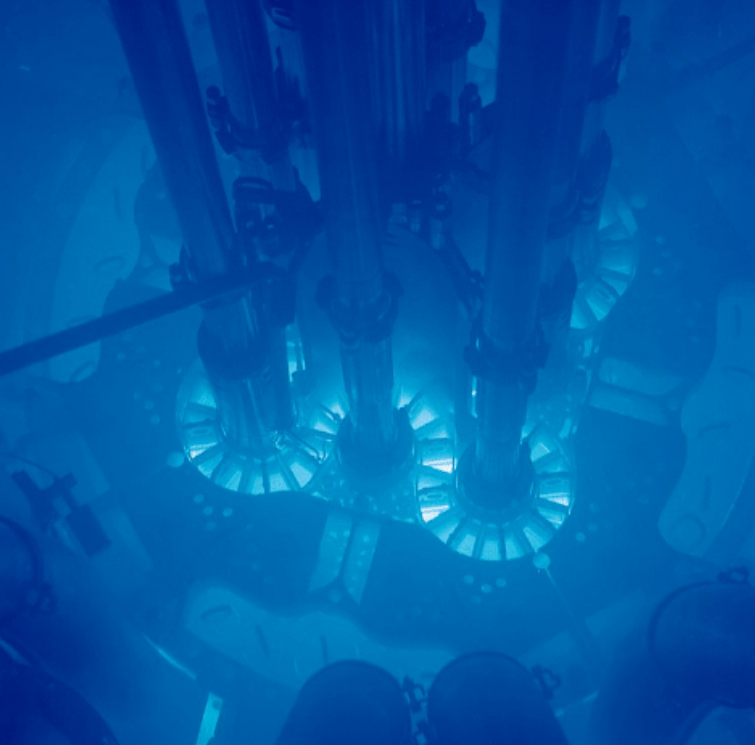
\includegraphics[width=0.25\textwidth]{images/reactor.PNG}}
  \caption{Schematic cherenkov radiation (a) and blue glow of an underwater nuclear plant (b).}
  \end{figure}
\end{frame}

\begin{frame}{Cherenkov radiation}
  \begin{itemize}
    \item Asymmetric polarisation of the medium results in a radiation of light due to relaxation
    \medskip
    \item Intensity is approximately proportional to the frequency of the light in the visible spectrum \\
    \rightarrow Cherenkov radiation is seen as blue
    \medskip
    %\item Occurrence of Cherenkov radiation:
      %\begin{itemize}
      %  \item Cosmic ray and high-energy photons can interact with the atmosphere and create electron-positron pairs with high velocities
      %  \medskip
      %  \item In pool-type nuclear reactors high-energy electrons are released as the fission products decay
      %  \medskip
      %  \item Imaging substances in a body through positron/beta emitters ($^{18}F$, $^{32}P$)
      %\end{itemize}
  \end{itemize}
  \begin{figure}
    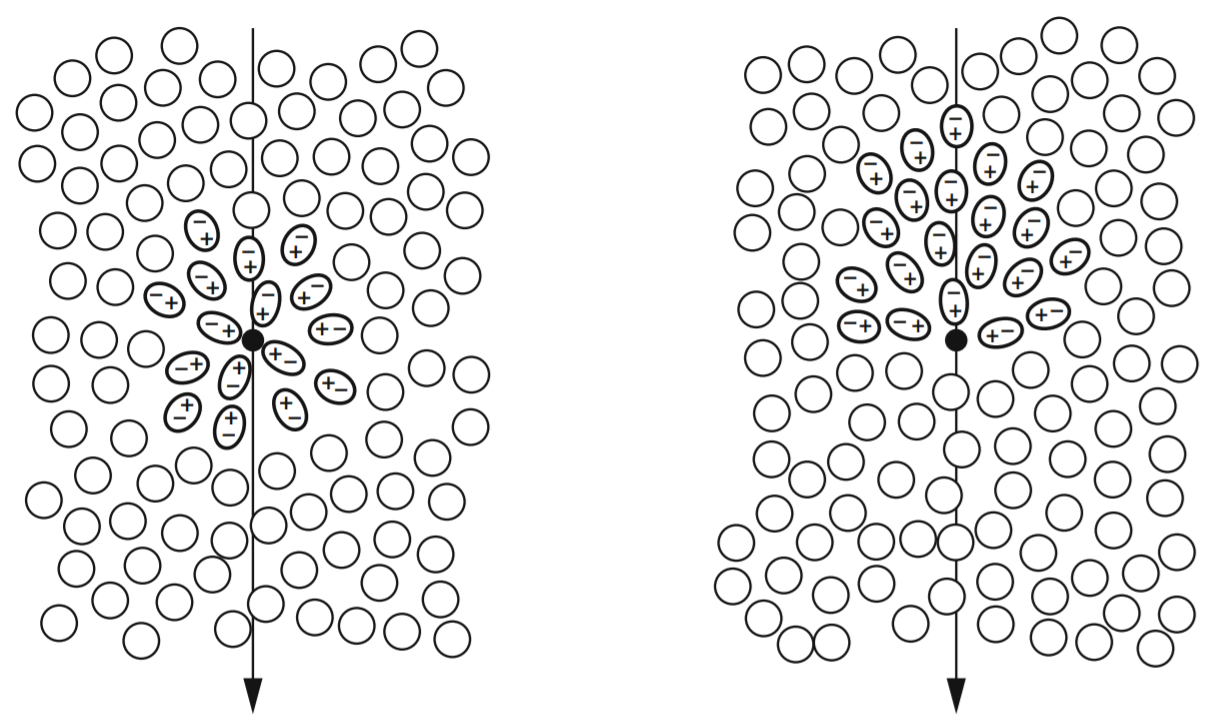
\includegraphics[width=0.4\textwidth]{images/polarisation.png}
    \caption{Polarisation of a dielectric medium at a particle velocity smaller (left) and greater (right) than the speed of light.}
  \end{figure}
\end{frame}



\begin{frame}{The first constructed Cherenkov detector}
  \begin{itemize}
    \item First Cherenkov counter was developed by J. V. Jelley in 1951
    \medskip
    \item Used to detect cosmic rays with high enough energy to produce Cherenkov light in water
    \medskip \\
  \end{itemize}
\vspace{0.5cm}
How it works:
  \begin{itemize}
    \item Distilled water in a cylinder functions as the radiator
    \medskip
    \item One side of the cylinder is connected to a photomultiplier
    \medskip
    \item Followed by a preamplifier to increase the signals
    \medskip
    \item Detector is direction sensitive as Cherenkov light ist only emitted in the foward direction
  \end{itemize}
\end{frame}

\begin{frame}{The first Cherenkov detector}
  \begin{figure}
    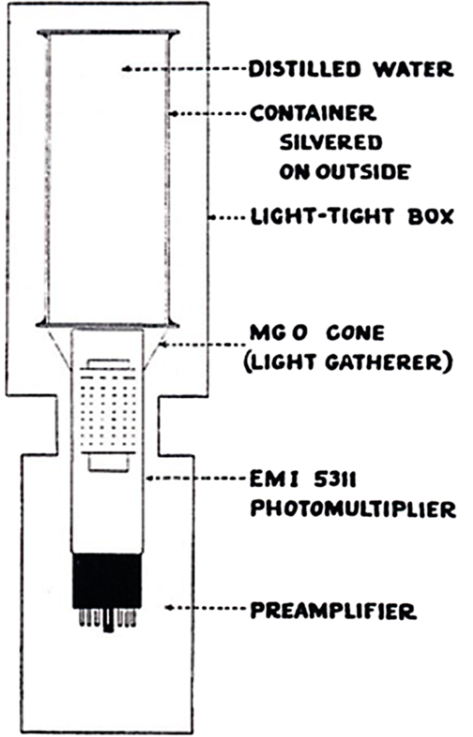
\includegraphics[width=0.28\textwidth]{images/the_first.png}
    \caption{Shematic representation of the first Cherenkov counter to measure cosmic ray.}
  \end{figure}
\end{frame}

\begin{frame}{Cherenkov light in the atmosphere}
  \begin{figure}
    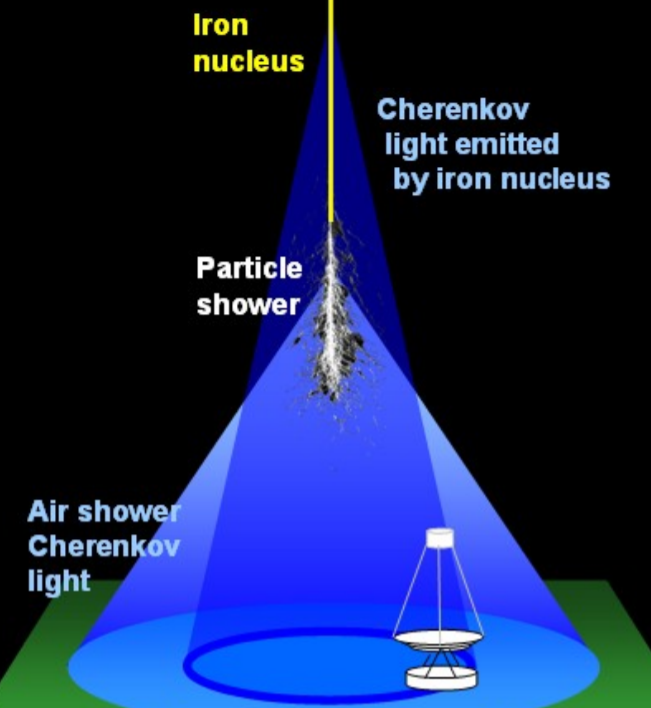
\includegraphics[width=0.35\textwidth]{images/cherenkov_cone.png}
    \caption{Shematic representation of an iron nucleus producing an air shower and cherenkov light.}
  \end{figure}
\end{frame}

\begin{frame}{The first Cherenkov detector in a particle accelerator}
  \begin{itemize}
    \item Used to detect single particles at the Birmingham proton synchrotron in 1956
    \medskip
    \item Was designed by Ivan A. Getting at MIT in 1947
  \end{itemize}

How it works:
\begin{itemize}
  \item A cone (acrylic plastic) with a top angle $\Phi$ functions as radiator
  \medskip
  \item Only Cherenkov light emitted at an angle $\Theta = \Phi$ will be focused by the lens through the collimator and measured by the
  photomultiplier (used for detection 0f 950 Mev protons)
\end{itemize}
\begin{figure}
  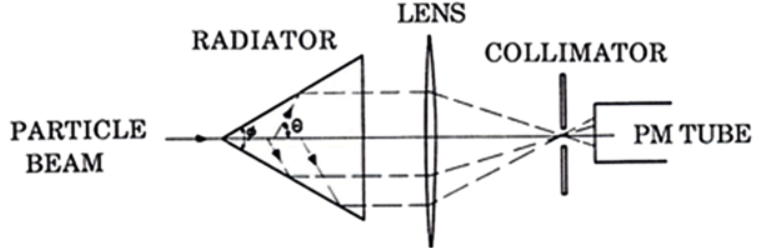
\includegraphics[width=0.55\textwidth]{images/the_second.png}
  %\caption{Shematic representation of the first Cherenkov counter to measure particles in a particle accelerator.}
\end{figure}
\end{frame}

\begin{frame}{Threshold detectors}
  \begin{itemize}
    \item Velocity of light in a medium decreases with increasing refractive index of the medium
    \medskip
    \item Threshold detectors use specific mediums to distinguish different particles
    \medskip
    \item Discovery of the antiproton was due to the help of a threshold detector in the proton synchrotron Bevatron in 1955
  \end{itemize}
  \begin{figure}
    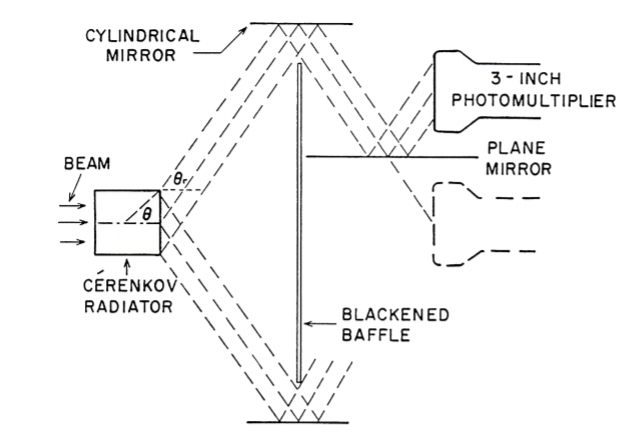
\includegraphics[width=0.39\textwidth]{images/proton.png}
    \caption{Cherenkov detector designed and used by Owen
     Chamberlain and Emilio Segré (Nobel Prize 1959), as well as Thomas Ypsilantis and Clyde Wiegand.
     Pions radiated Cherenkov light in the fused quartz, while antiprotons did not.}
  \end{figure}
\end{frame}


\begin{frame}{Differential Cherenkov detector}
  \begin{itemize}
    \item Uses the angle of the cherenkov cone to focus light through a diaphragm
    \medskip
    \item Measurable velocity range is dependant on radius of diaphragm
    \medskip
    \item Refractive index of a gas radiator can be controlled through pressure
  \end{itemize}
    \begin{figure}
      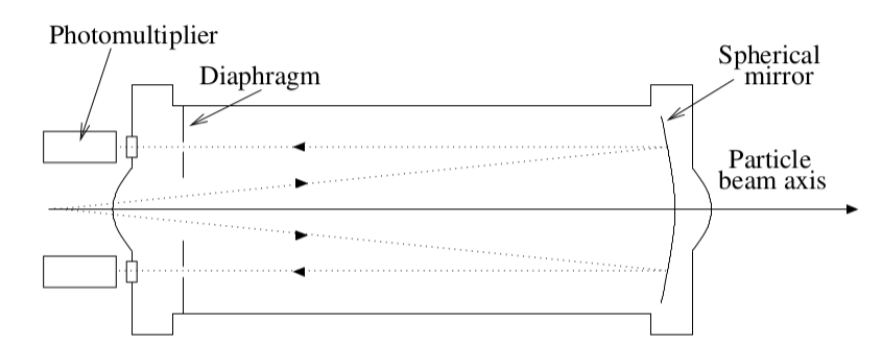
\includegraphics[width=0.6\textwidth]{images/differential.png}
      \caption{Predecessor of Ring Imaging Cherenkov detectors. Range of velocity measurement can be controlled through
      gas radiators and the diaphragm.}
    \end{figure}
\end{frame}

\begin{frame}{Ring Imaging Cherenkov (RICH) detector}
  \begin{itemize}
    \item First Cherenkov detector to measure velocity of particles
    \medskip
    \item J. S\'{e}guinot and T. Ypsilantis designed the first RICH detector in 1976
  \end{itemize}
\vspace{0.5cm}
How it works:
\begin{itemize}
  \item Consists of a spherical detector and mirror with a radiator inbetween
  \medskip
  \item Incoming particles emit Cherenkov light between detector and a mirror
  \medskip
  \item Light is reflected onto photo sensitive detector
  \medskip
  \item Ring shaped reflections enable calculation of velocity ($\Theta = 2 \frac{R_c}{R}$)
\end{itemize}
\end{frame}

\begin{frame}{First RICH detector}
  \begin{figure}
    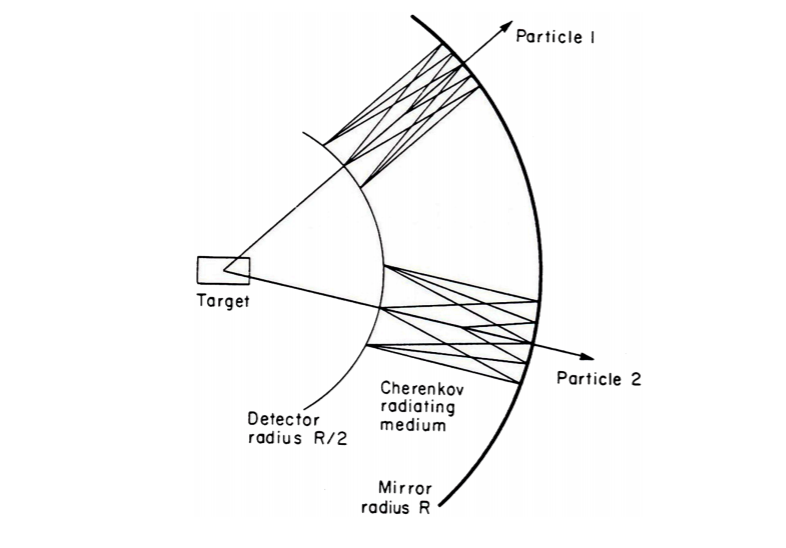
\includegraphics[width=0.55\textwidth]{images/rich.png}
    \caption{Shematic representation of the first Ring Imaging Cherenkov detector.}
  \end{figure}
\end{frame}

\begin{frame}{Modern RICH detector}
  \begin{itemize}
    \item Used in the DELPHI experiment at cern until 2001
    \medskip
    \item RICH detector worked with two radiators to cover a larger momentum range (0.5-40 GeV/c)
  \end{itemize}
  \begin{figure}
    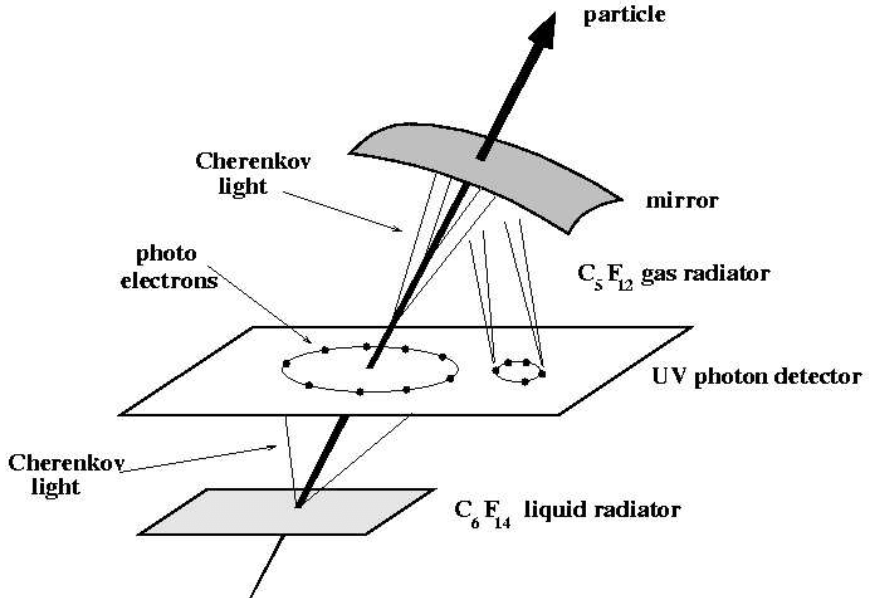
\includegraphics[width=0.45\textwidth]{images/rich_delphi.png}
    \caption{RICH detector in the DELPHI experiment using two radiators and one photon detector. The Cherenkov light is projected on both
    sides of the detector.}
  \end{figure}
\end{frame}

\begin{frame}{The photon detector}
  \begin{itemize}
    \item Reconstruction of a ring can be challenging, especially with gas radiators (fewer photons)
    \medskip
    \item Photon detector must be able to localize the spatial position in the ring image
    %\medskip
    %\item Needs uniform sensitivity over a wide velocity range (no diaphragms)
  \end{itemize}
How it works:
\begin{itemize}
  \item Photons enter conversion region (commonly filled with a gas) and ionize an electron
  \medskip
  \item Electron drifts towards a multiwire proportional chamber (measurement of two coordinates)
  \medskip
  \item Last coordinate of the photon is calculated with the drift time of the electron
\end{itemize}
  \begin{figure}
    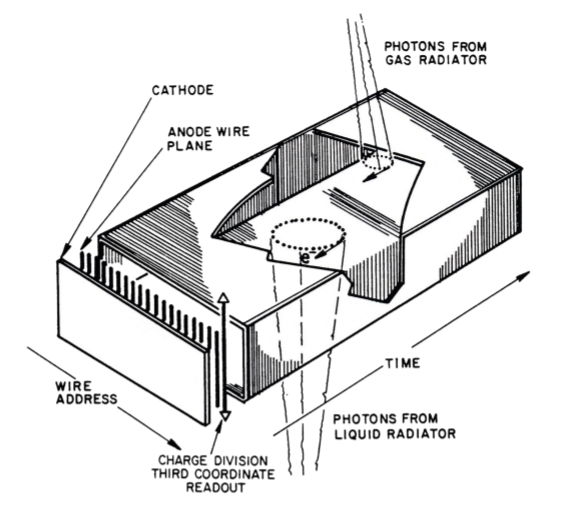
\includegraphics[width=0.3\textwidth]{images/photon_det.png}
    %\caption{Photon detector for RICH detectors. In the DELPHI experiment cathode strips measure one coordinate instead of a
    %charge division}
  \end{figure}
\end{frame}

\begin{frame}{The DELPHI experiment}
  \begin{figure}
    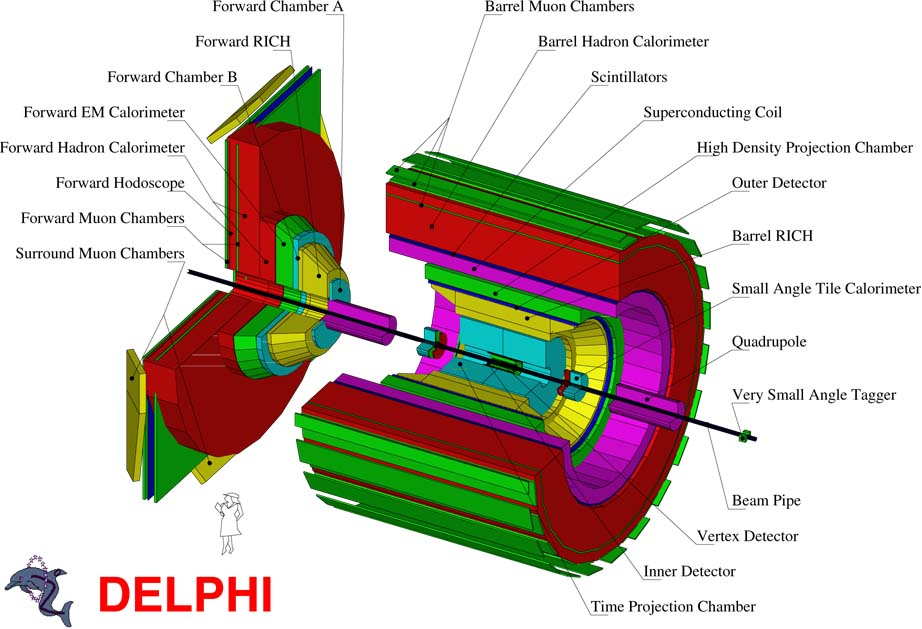
\includegraphics[width=0.55\textwidth]{images/delphi.jpg}
    \caption{Representation of the DELPHI experiment with it's components. The yellow zylindrical component is the RICH detector.}
  \end{figure}
\end{frame}

\begin{frame}{Detection of Internally Reflected Cherenkov light (DIRC)}
  \begin{itemize}
    \item A RICH detector used in the BaBar detector at SLAC (until 2008)
    \medskip
    \item Thin quartz radiator also functions as waveguide for the cherenkov light
    \medskip
    \item Identifies particles up to 4.2 GeV/c
  \end{itemize}
  \begin{figure}
    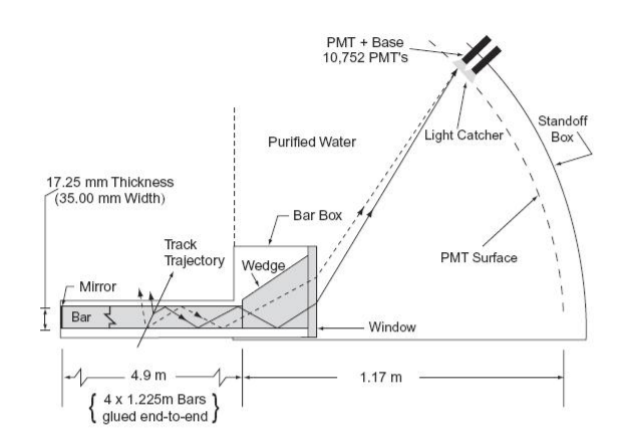
\includegraphics[width=0.45\textwidth]{images/dirc.png}
    \caption{Side view of the DIRC. With the Cherenkov angle and the momentum calculated with the tracking chambers, the
    particles mass can be determined}
  \end{figure}
\end{frame}

\begin{frame}{The BaBar experiment}
  \begin{figure}
    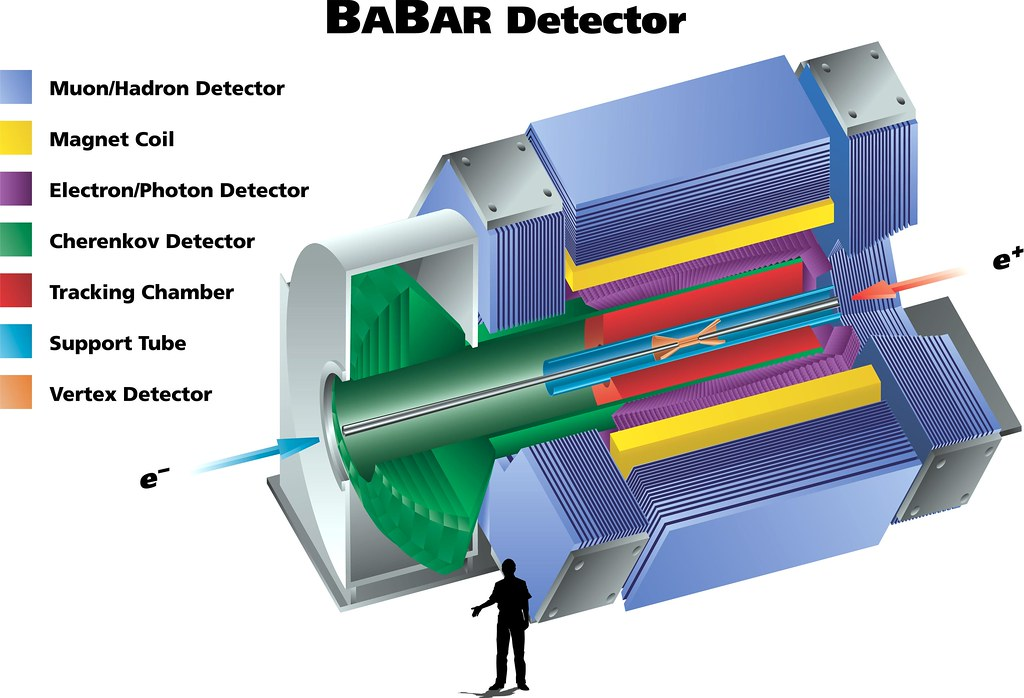
\includegraphics[width=0.55\textwidth]{images/babar.jpg}
    \caption{The BaBar experiment with it's components highlighted.}
  \end{figure}
\end{frame}

\begin{frame}{Imaging Atmospheric Cherenkov Telescope (IACT)}
  \begin{itemize}
    \item Telescopes to detect high energy gamma ray photons in the range of 50 GeV to 50 TeV
    \medskip
    \item First IACT (Whipple 10m Telescope) was developed by the Whipple collaboration in 1968
    \medskip
    \item Currently four operating IACT systems (MAGIC, VERITAS, MACE, H.E.S.S.)
  \end{itemize}
\vspace{0.5cm}
How they work:
\begin{itemize}
  \item Cherenkov light is reflected onto an array of photomultipliers with a large segmented mirror
  %\item Imaging of Cherenkov radiation generated by charged particles in an air shower
  \medskip
  \item Cherenkov flash illuminates many 100 $\mathrm{m}^2 \rightarrow$ Usage of more than one telescope approximately 100$\, \mathrm{m}$ apart to
  reconstruct the shower
\end{itemize}
\end{frame}



\begin{frame}{MAGIC and H.E.S.S.}
  \begin{figure}
      \subfigure[]{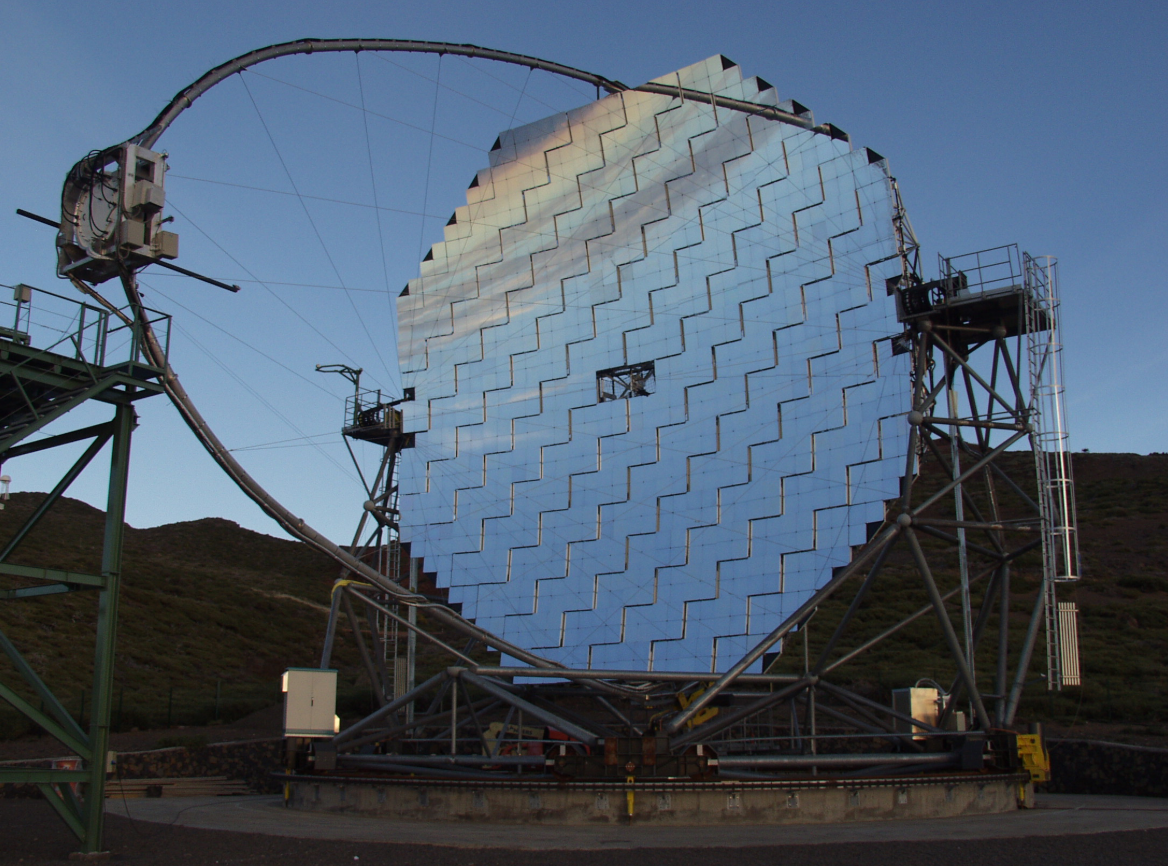
\includegraphics[width=0.48\textwidth]{images/magic.PNG}}
      \hspace{0.5cm}
      \subfigure[]{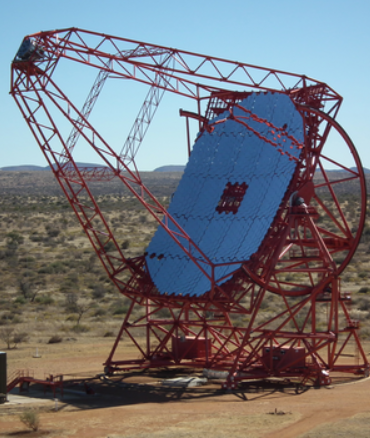
\includegraphics[width=0.3\textwidth]{images/hess.PNG}}
  \caption{ The MAGIC telescope (a) and the H.E.S.S. telescope (b).}
  \end{figure}
\end{frame}


\begin{frame}{IceCube}
  \begin{itemize}
    \item Neutrino observatory at the Amundsen–Scott South Pole Station in Antarctica (completed in 2010)
    \medskip
    \item Measures high energy neutrinos in the range of 100 GeV to several PeV
  \end{itemize}
\vspace{0.5cm}
  How it works:
  \begin{itemize}
    \item $1 \: \mathrm{km}^3$ of ice functions as radiator
    \medskip
    \item Neutrinos can interact with ice, creating large leptons (e.g. $\bar{\nu}_e + p \rightarrow e^{+} + n$)
    \medskip
    \item Charged leptons can radiate Cherenkov light, which are measured by photomultipliers
    \medskip
    \item IceTop is a Cherenkov detector at the surface to detect cosmic ray particles
    \medskip
    \item The Deep Core strings are able to measure Neutrinos at lower energies than 100 GeV
  \end{itemize}
\end{frame}

\begin{frame}{IceCube}
  \begin{figure}
    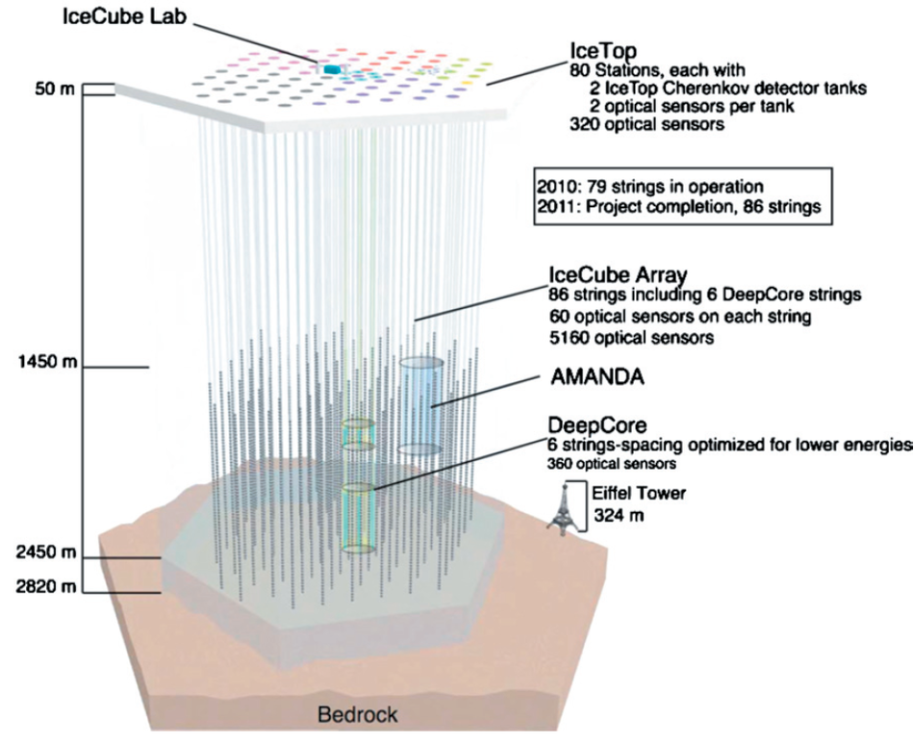
\includegraphics[width=0.55\textwidth]{images/icecube.png}
    \caption{Structure of the neutrino detector IceCube.}
  \end{figure}
\end{frame}


\begin{frame}{Super-Kamiokande}
  \begin{itemize}
    \item Cylindrical water tank with 40 m height and diameter in Japan (operates since 1996)
    \medskip
    \item Functions similar to IceCube
    \medskip
    \item Nobel Prize for proof of neutrino oscillation (2015)
  \end{itemize}
  \begin{figure}
    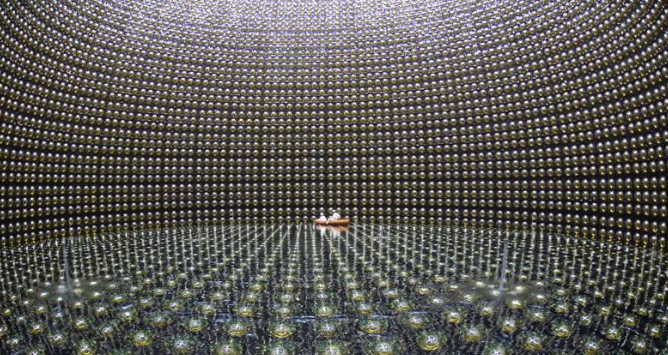
\includegraphics[width=0.5\textwidth]{images/kamiokande.png}
    \caption{Inside of Super-Kamiokande, 1000 meter underground, with 13000 photomultipliers.}
  \end{figure}
\end{frame}

%\begin{frame}{}



%\begin{frame}{References}
%  \item https://www.mpi-hd.mpg.de/hfm/HESS/pages/about/telescope
%  \item Position sensitive gaseous photomultipliers: Research and apllications
%I. Adam et al. /Nuclear Instruments and Methods in Physics Research A 538 (2005)
%\end{frame}

\end{document}
